\documentclass[12pt,a4paper]{article}
\usepackage[utf8]{inputenc}
\usepackage{amsmath}
\usepackage{amsfonts}
\usepackage{amssymb}
\usepackage{graphicx}
\usepackage{setspace}
\usepackage{nicefrac}
\usepackage{bbold}
\usepackage{booktabs} % toprule, midrule, ..
\usepackage[left=2.00cm, right=2.00cm, top=2.00cm, bottom=2.00cm]{geometry}
\usepackage{siunitx}
\usepackage{url}
\usepackage{paralist}
\usepackage{enumitem} % special labels
\usepackage{multirow}
\usepackage{rotating}

\usepackage{minted}

\usepackage{longtable,tabu}

\usepackage{multicol,multirow}
\usepackage{tikz}

\usepackage{hhline}
\usepackage{placeins}

\usetikzlibrary{shapes,snakes,trees}

\definecolor{mintedbg}{rgb}{.97,.97,1.}
\setminted{breaklines,bgcolor=mintedbg}

\title{Project: Bubble Bobble\\Phase 3}
\author{Pierre Beaujean}
\date{Due for May 6$^\text{th}$, 2018}

\setlength{\jot}{10pt} % aligns
\renewcommand{\arraystretch}{1.1}
\setlength{\tabcolsep}{0.20cm}
\onehalfspacing

\newcommand{\cc}[1]{\mintinline{c}{#1}}

\begin{document}
\maketitle

\section{Introduction}

Bubble Booble, released in 1986 by Taito in arcades, is an action platformer type video game where the player controls two dragons, named Bub (green) and Bob (blue). To save their girlfriends, kidnapped in the last stage of the game, the dragons must go through different levels by blowing bubbles to trap their enemies, then burst them. When they do, they create items that, if collected, give them a certain amount of point (and may get heal and extra life, depending on the object). If there are no more monsters to trap, the dragons go to the next one after a given amount of time (or if all the items have been collected). One level is limited to a single screen, constituted of platforms (and walls in the left and the right of the screen). The dragons can move along the platform, jump over higher ones and fall to lower ones. Note that if the dragon fall into a gap in the bottom of the screen, it reappears on the top. Monsters chase the dragons, which loses one life (out of 3, but some items give extra lives) if touched by the monster. If the player takes too much time to complete a level, an extra monster (initially an invincible one) is added to the level \cite{wikibub,wikibub2}.

Note that the original arcade game displays a bit more complexity than the playable version available on the Internet, for example in 8bbits \cite{playbub}, which correspond to the NES version. During this work, I will therefore reproduce this NES version that I was able to play in order to understand the different game mechanistic. A list of the modification with respect to the original version is available in StrategyWiki \cite{wikibub2_nes}.

The goal of this report is to present an implementation of the game, realized during this first year of Bachelor in the frame of the \textit{Programmation II} lecture. This implementation contain all the basic game mechanism described above, with multiple playable levels and a score counter, but is a one-player version (with Bub).

\section{Game specifications}

The following part will detail different aspects of the game implementations, starting by the screens, then the data structures and finally some explanation on which functions are needed to implement the game logic.

\subsection{Screens}

Following the original NES game, the program window is a square of 512$\times$432 px.\footnote{This is actually twice the size of the original screen, but on modern screen, that's a minimum if ones want to see something!}

The welcome screen is given in Figure \ref{fig:1:welcome}. To simplify a bit with respect to the original game, it presents both the game title and options. The options are given in the form of a list and a cursor allow to select the options.

\begin{figure}[!h]
	\centering
	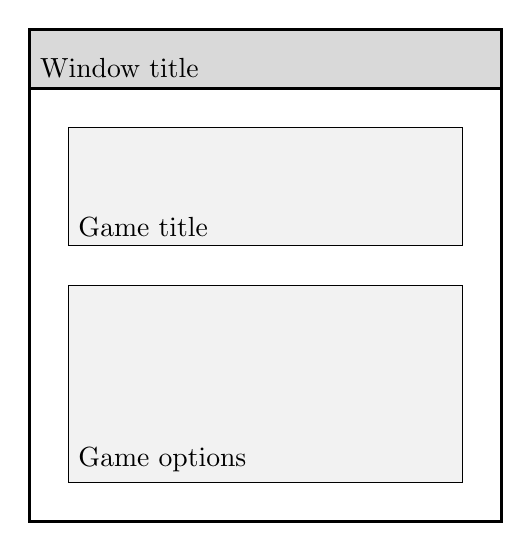
\begin{tikzpicture}
	\draw[very thick,fill=black!15] (0,5.5) node[anchor=south west]{Window title} rectangle +(6,.75);
	\draw[very thick] (0,0)  rectangle +(6,5.5);
	\draw[fill=black!5] (.5,3.5) node[anchor=south west]{Game title} rectangle +(5,1.5);
	\draw[fill=black!5] (.5,.5) node[anchor=south west]{Game options} rectangle +(5,2.5);
	\end{tikzpicture}\hspace{.5cm}
	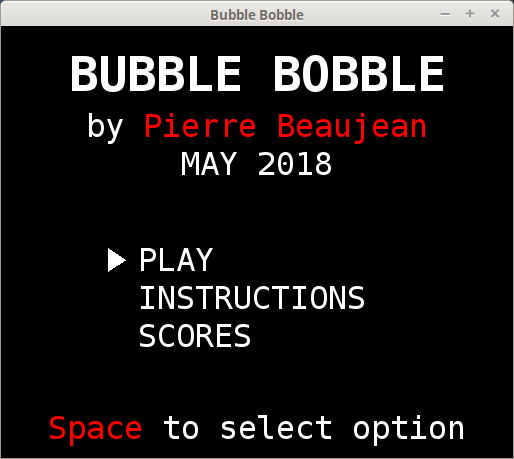
\includegraphics[width=.45\linewidth]{i/screen1}
	
	\caption{Welcome screen of the game (sketch on the left, actual implementation on the right).}
	\label{fig:1:welcome}
\end{figure}

The control screen is given in Figure \ref{fig:2:controls}: there is a title to indicate what the player sees, and some text.

\begin{figure}[!h]
	\centering
	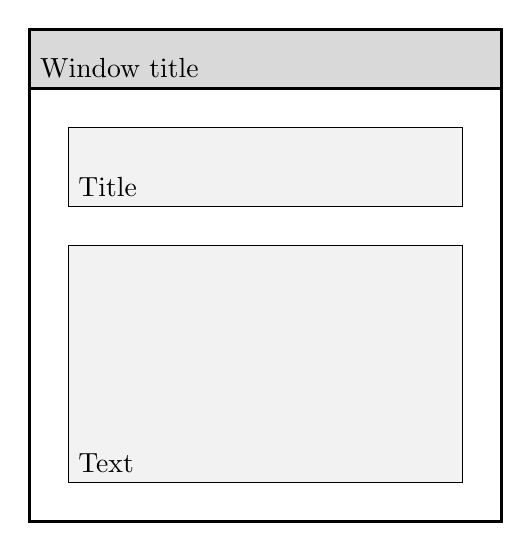
\begin{tikzpicture}
	\draw[very thick,fill=black!15] (0,5.5) node[anchor=south west]{Window title} rectangle +(6,.75);
	\draw[very thick] (0,0)  rectangle +(6,5.5);
	\draw[fill=black!5] (.5,4) node[anchor=south west]{Title} rectangle +(5,1);
	\draw[fill=black!5] (.5,.5) node[anchor=south west]{Text} rectangle +(5,3);
	\end{tikzpicture}\hspace{.5cm}
		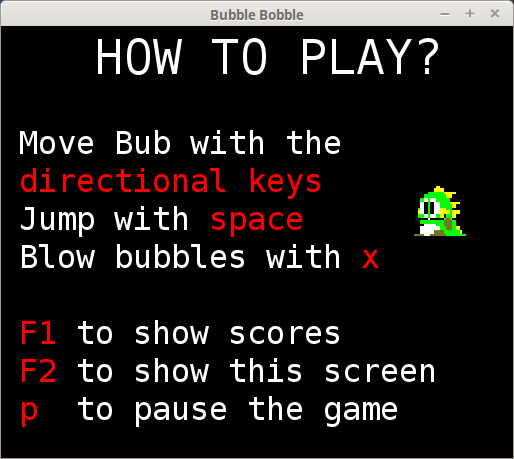
\includegraphics[width=.45\linewidth]{i/screen2}
	\caption{Controls and score screen of the game (sketch on the left, actual implementation on the right).}
	\label{fig:2:controls}
\end{figure}

The score screen is given in Figure \ref{fig:3:score}. In this screen, the score are continuously going up, and the list is repeated. 

\begin{figure}[!h]
	\centering
	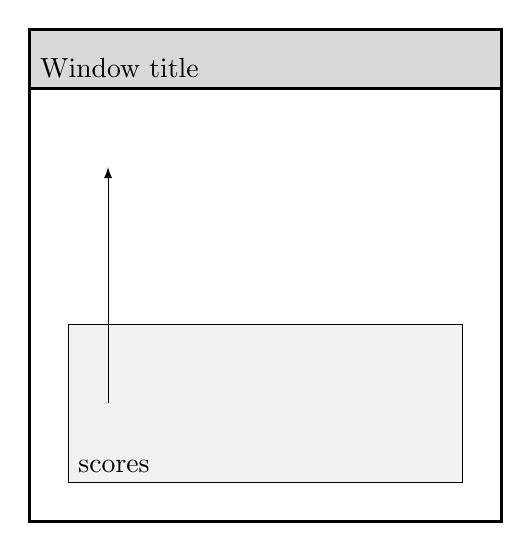
\begin{tikzpicture}
	\draw[very thick,fill=black!15] (0,5.5) node[anchor=south west]{Window title} rectangle +(6,.75);
	\draw[very thick] (0,0)  rectangle +(6,5.5);
	\draw[fill=black!5] (.5,.5) node[anchor=south west]{scores} rectangle +(5,2);
	\draw [-latex] (1,1.5) -- +(0, 3);
	\end{tikzpicture}\hspace{.5cm}
		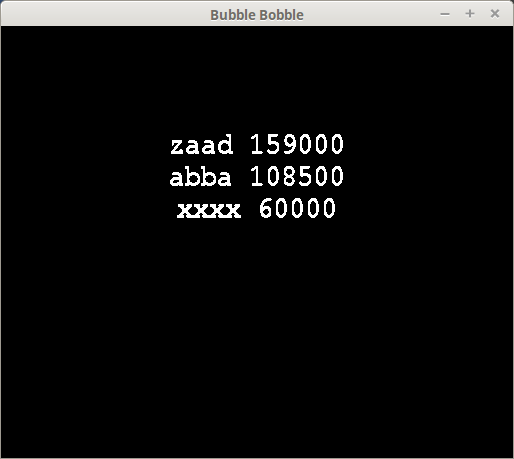
\includegraphics[width=.45\linewidth]{i/screen3}
	\caption{Score screen of the game (sketch on the left, actual implementation on the right).}
	\label{fig:3:score}
\end{figure}

The game over/final screen is given in Figure \ref{fig:3:gameover}. This screen gives the possibility to enter a name associated with the score. If it is game over, the possibility to save the score is not given.

\begin{figure}[!h]
	\centering
	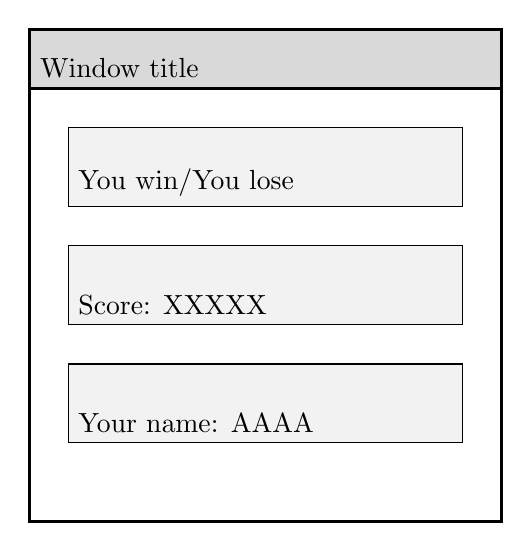
\begin{tikzpicture}
	\draw[very thick,fill=black!15] (0,5.5) node[anchor=south west]{Window title} rectangle +(6,.75);
	\draw[very thick] (0,0)  rectangle +(6,5.5);
	\draw[fill=black!5] (.5,4) node[anchor=south west]{You win/You lose} rectangle +(5,1);
	\draw[fill=black!5] (.5,2.5) node[anchor=south west]{Score: XXXXX} rectangle +(5,1);
	\draw[fill=black!5] (.5,1) node[anchor=south west]{Your name: AAAA} rectangle +(5,1);
	%\draw[fill=black!5] (.5,.5) node[anchor=south west]{Text} rectangle +(5,3);
	\end{tikzpicture} \\
	\vspace{.5cm}
			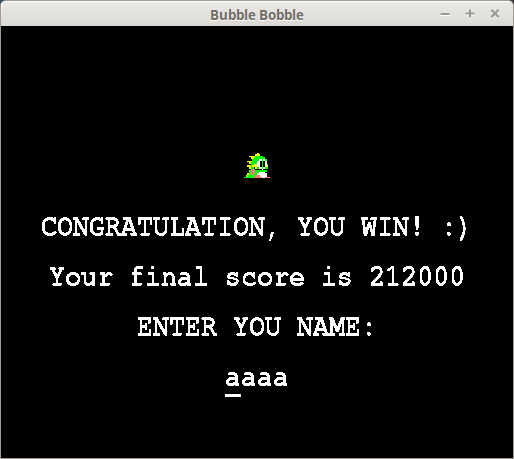
\includegraphics[width=.45\linewidth]{i/screen4}\hspace{.5cm}
			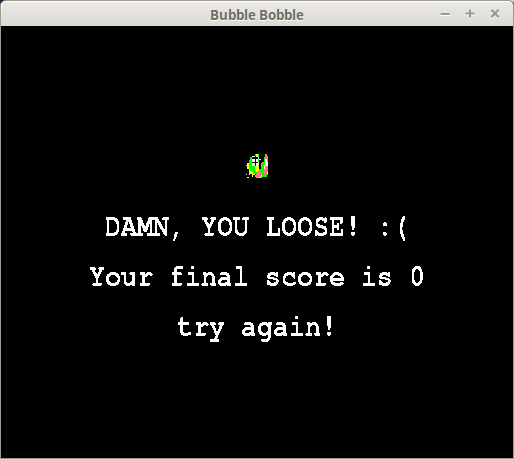
\includegraphics[width=.45\linewidth]{i/screen4b}
	\caption{Game over/final screen of the game (sketch on top, actual implementation on bottom). The player can associate a (four letters) name to its score.}
	\label{fig:3:gameover}
\end{figure}

Finally, the game screen is given in Figure \ref{fig:4:game}. This screen is subdivided in 32$\times$27 squares of 16$\times$16 px (the two top rows being outside of the actual gaming area). Each square is either \textbf{empty} (black) or \textbf{filled} (with a tile image), to represent a physical wall/platform. An actual map is actually 32$\times$24, since the last line is exactly the same as the first one (so that if a dragon/monster fall in the bottom, it can reappear in the top). A map object (item, dragon, monster) is a $2\times2$ square.

%A dragon or a monster move by one square at the time on the left and the right, if there is no filled square in the way. Its jump is of 6 squares up. When it jumps, the dragon/monster  goes up first (whether or not there is filled squares in the way), then go down and stops in an empty square, if there is a filled square below (otherwise, it continues to fall). The position of Bub is always the same at the beginning of the level and when they lose a life (see Figure \ref{fig:4:game}). The position of the monster depends on the level (at the beginning of the level, they fall from the top to a given position in the level, then starts to move).

% The movement of a bubble is very specific: it starts by going in the direction it has been blown, until it loses its \textit{momentum}. When it does, all the bubbles end up in about the same position in the level, by going up/down first, then left/right. Bubbles burst on their own after a time, freeing the monster that they contain if it was the case.

\begin{figure}[!h]
	\centering
	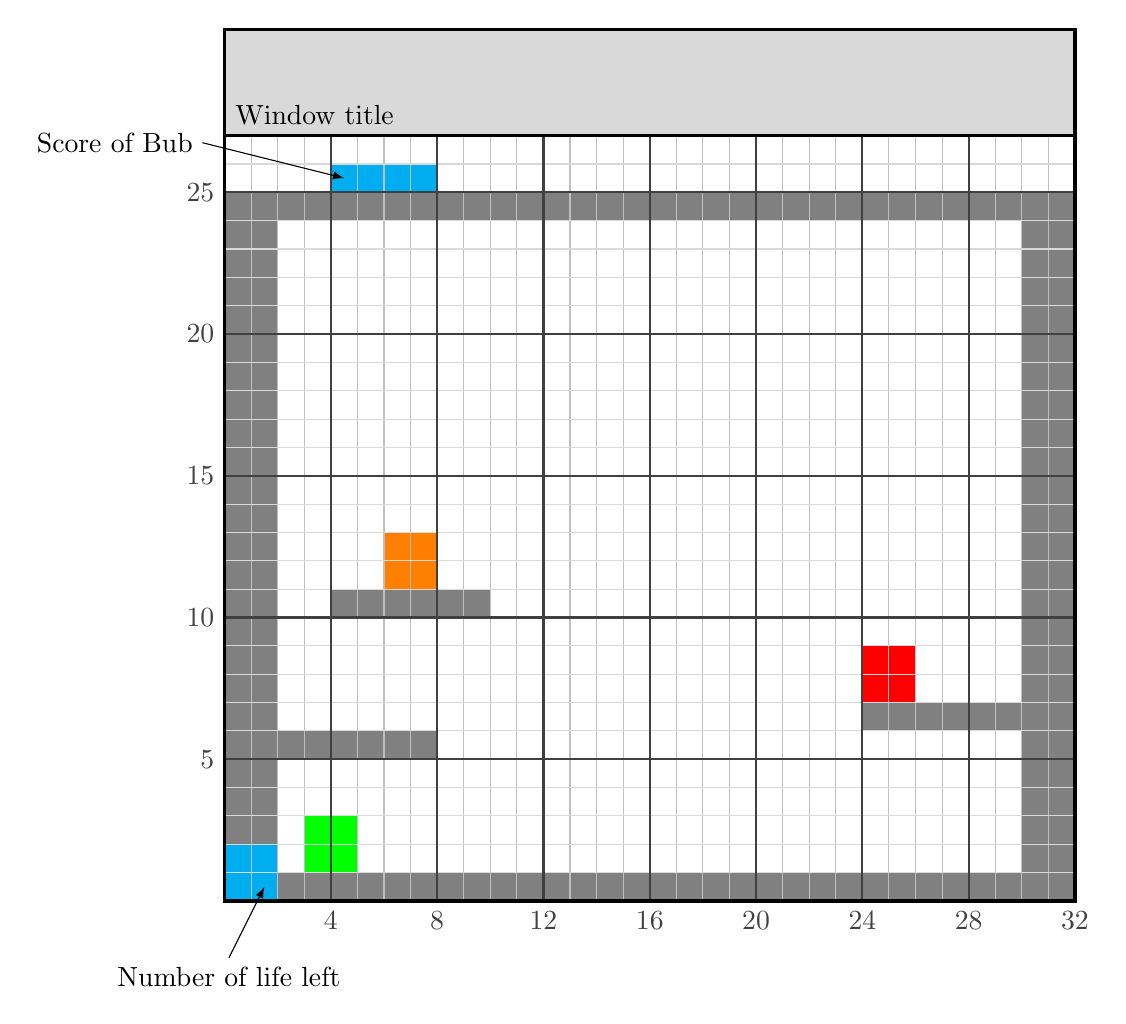
\begin{tikzpicture}[scale=.9]
	% wall
	\fill[black!50] (0,0) rectangle +(.75,10);
	\fill[black!50] (11.25,0) rectangle +(.75,10);
	\fill[black!50] (.75,0) rectangle +(11.25,.4);
	\fill[black!50] (.75,9.6) rectangle +(11.25,.4);
	
	% platform
	\fill[black!50] (.75,2) rectangle +(2.25,.4);
	\fill[black!50] (1.5,4) rectangle +(2.25,.4);
	
	\fill[black!50] (9,2.4) rectangle +(2.25,.4);
	
	% bub&bob
	\filldraw[green] (1.125,.4) rectangle +(.75,.8);
	%\filldraw[blue] (10.125,.4) rectangle +(.75,.8);
	
	% monster & item
	\filldraw[orange] (2.25,4.4) rectangle +(.75,.8);
	\filldraw[red] (9.,2.8) rectangle +(.75,.8);
	
	% info
	\filldraw[cyan] (0,0) rectangle +(.75,.8);
	%\filldraw[cyan] (11.25,0) rectangle +(.375,.4);
	
	\filldraw[cyan] (1.5,10) rectangle +(1.5,.4);
	
	%\filldraw[cyan] (9,10) rectangle +(1.5,.4);
	
	%\filldraw[cyan] (5.625,9.6) rectangle +(.75,.4);
	
	% grid
	\foreach \i in {1,2,...,31}{
		\draw[black!25] (\i*.375,0) -- +(0,11);
	}  
	\foreach \i in {1,2,...,26}{
	\draw[black!15] (0,.4*\i) -- +(12,0);
	} 

	\foreach \i in {4,8,...,32}{
	\draw[black!75,thick] (\i*.375,0) node[below]{\i} -- +(0,11);
	}  
	\foreach \i in {5,10,...,25}{
		\draw[black!75,thick] (0,.4*\i) node[left]{\i} -- +(12,0);
	} 

	\draw[very thick,fill=black!15] (0,10.8) node[anchor=south west]{Window title} rectangle +(12,1.5);
	\draw[very thick] (0,0)  rectangle +(12,10.8);
	
	\draw[latex-] (.375+.5*.375,0+.2) -- +(-.5,-1) node[below]{Number of life left};
	%\draw[latex-] (11.25+.5*.375,0+.2) -- +(.5,-1) node[below]{Number of life left (Bob)};
	\draw[latex-] (1.5+.5*.375,10+.2) -- +(-2,.5) node[left]{Score of Bub};
	%\draw[latex-] (10.125+.5*.375,10+.2) -- +(2,.5) node[right]{Score of Bob};
	%\draw[latex-] (5.625+.5*.375,9.6+.2) -- +(0,3) node[above]{Level number};
	
	\end{tikzpicture}
	
	\vspace{.5cm}
	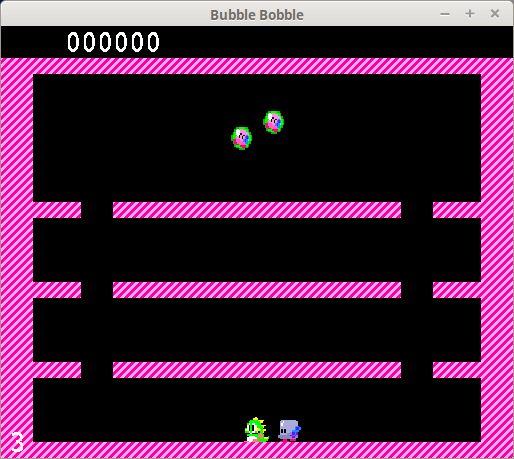
\includegraphics[width=.5\linewidth]{i/screen5}
	
	\caption{Game screen (sketch on top, actual implementation on bottom) subdivided in 32$\times$27 squares. Filled square represent walls/platform. The starting position of Bub is represented by the green square. The orange square represents an item, which Bub is able to grab by jumping on the first, then the second platform (since they are spaced by 5 squares), while Bob will not be able to reach the platform on top of him (since it is 6 squares up). On the other hand, the monster (red square) is able to jump down and try to touch Bob. The position of some extra information (score, life left) is given in lighter blue.}
	\label{fig:4:game}
\end{figure}


\subsection{Modules: data structures and main functions}

\subsubsection{Preamble: conventions}

\begin{figure}[!p]
\centering
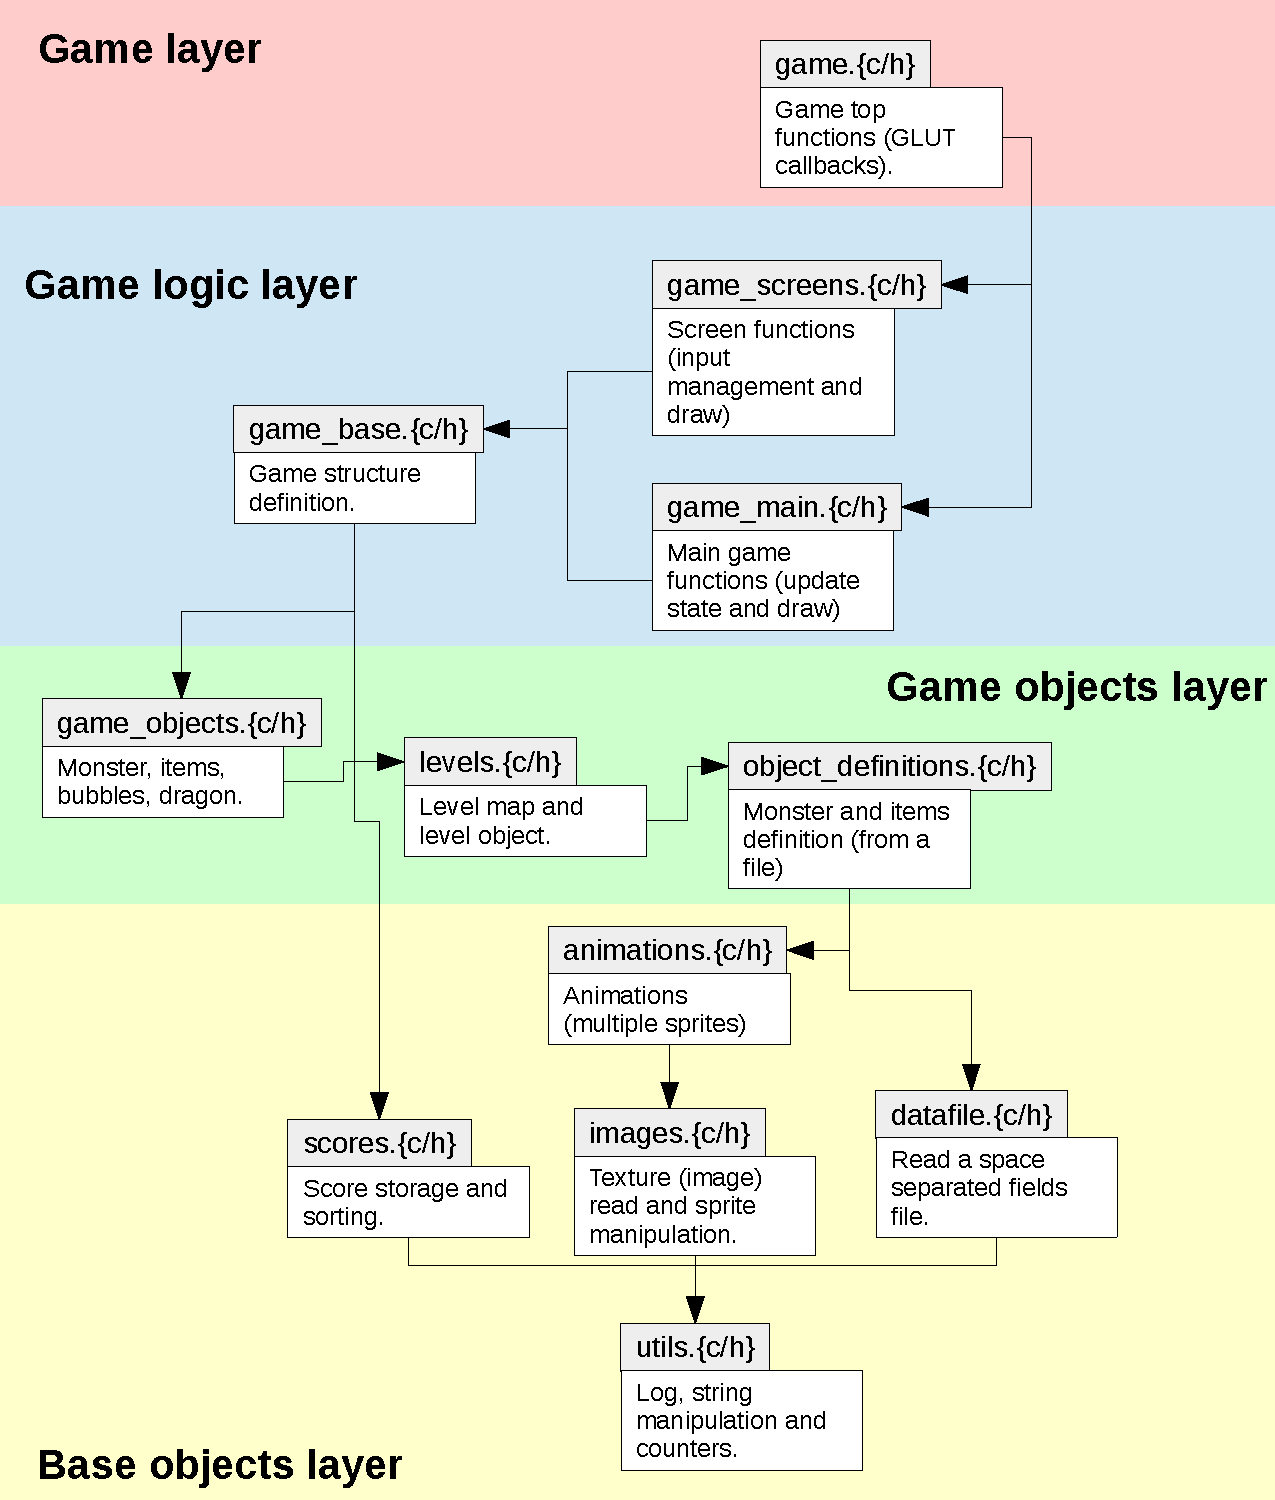
\includegraphics[width=.8\linewidth]{i/files}
\caption{Module organization and main features of those modules. The arrows show what is included in each module.}
\label{fig:modules}
\end{figure}

The following parts will follow these conventions:

\begin{itemize}
\item The module (divided into 4 layers) are organized as presented in Figure \ref{fig:modules}. The bottom layer contains all the methods and structure for basic manipulation (of images, files and score). Then, the game object layer contains methods and structures that make sense in the game (the map, the monsters, the bubbles, the items and the dragon). The following layer (game logic) gathers all the objects together and deals with how they interact together, as well as their responses to inputs (only for the dragon or the screens). Finally, the last layer (game) contains the interactions with GLUT (with all the callbacks that it needs). The following pages will present the different modules from the bottom to the top.
\item The \cc{*_new()}  (and \cc{*_new_from_file()}) type functions will perform the necessary \cc{malloc()} and initialize the structure(s), while the \cc{*_delete()} type functions will perform the required \cc{free()}'s. 
\item The \cc{*_copy()} type functions copy a structure to another, and take care to copy the element of the structure correctly (by using the corresponding copy functions if needed). This is needed since you need to be sure that the element is destroyed only when the structure is.
\item  The \cc{blit_*()} type functions simply ``blit" (draw\footnote{This term comes from another C graphic library, the SDL.}) the object on the screen, using a sprite or an animation (see below). 
\item The program will log a certain number of informations in order to be able to detect and fix a crash.
\item A chained list corresponds to the following representation:\begin{center}
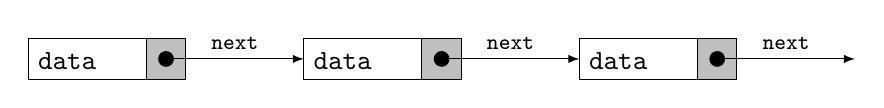
\begin{tikzpicture}
\foreach\i in {0,1,2} {
\begin{scope}[xshift=\i*3.5cm]
\draw (0,0) node[anchor=south west]{\texttt{data}} rectangle +(1.5,1.5em);
\draw[fill=black!25] (1.5,0) rectangle +(.5,1.5em);
\fill (1.75,.75em) circle (.1cm);
\draw[-latex] (1.75,.75em) -- node[above]{\footnotesize\texttt{next}} +(1.75,0);
\end{scope}
}
\end{tikzpicture}
\end{center}
where \cc{data} is a block of data and \text{next} a pointer to the next element of the list. It is a \cc{NULL} terminated chained list if the last element is set to \cc{NULL}, while it is circular if the last element point to the first element of the chain. Notice that in the case of circular lists, a sentinel is needed: \begin{center}
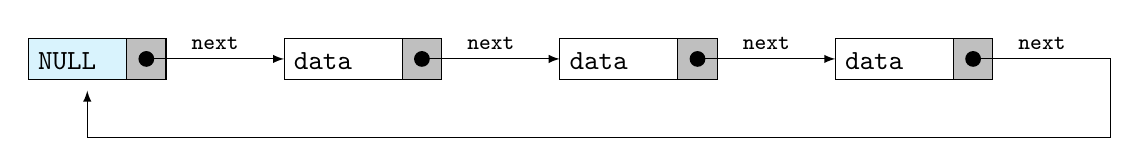
\begin{tikzpicture}
\draw[fill=cyan!15]  (-3.25,0) node[anchor=south west]{\texttt{NULL}} rectangle +(1.5,1.5em);
\draw[fill=black!25] (-2,0) rectangle +(.5,1.5em);

\foreach\i in {0,1,2} {
\begin{scope}[xshift=\i*3.5cm]
\draw (0,0) node[anchor=south west]{\texttt{data}} rectangle +(1.5,1.5em);
\draw[fill=black!25] (1.5,0) rectangle +(.5,1.5em);
\fill (-1.75,.75em) circle (.1cm);
\draw[latex-] (0,.75em) -- node[above]{\footnotesize\texttt{next}} +(-1.75,0);
\end{scope}
}
\fill (8.75,.75em) circle (.1cm);
\draw[-latex] (8.75,.75em) -- node[above]{\footnotesize\texttt{next}} ++(1.75,0) -- ++(0,-1) -- ++(-13, 0) -- ++(0,1.7em);
\end{tikzpicture}
\end{center}
The sentinel (blue in the scheme above) is always the first element of the list, and the data is set to \cc{NULL}.
\item All files used here (except image files) will be text files. Each of these files will contain multiple lines with values in it. Each value is space-separated. To define a file format, the following representation will be used:\begin{center}
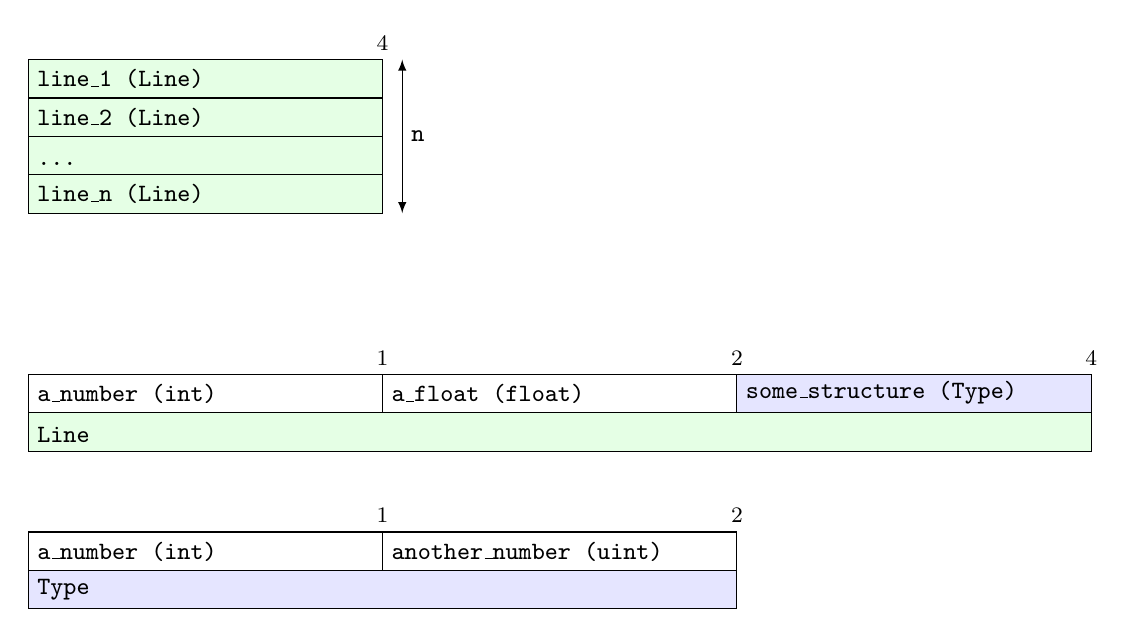
\begin{tikzpicture}
\small
\def\sz{4.5}

\draw[fill=green!10] (0,4) node[anchor=south west]{\texttt{line\_1 (Line)}} rectangle +(\sz,1.5em) node[above]{\footnotesize 4};
\draw[fill=green!10] (0,4cm-1.5em) node[anchor=south west]{\texttt{line\_2 (Line)}} rectangle +(\sz,1.5em);
\draw[fill=green!10] (0,4cm-3em) node[anchor=south west]{\texttt{...}} rectangle +(\sz,1.5em);
\draw[fill=green!10] (0,4cm-4.5em) node[anchor=south west]{\texttt{line\_n (Line)}} rectangle +(\sz,1.5em);

\draw[latex-latex] (\sz cm+.25cm,4cm+1.5em) -- node[right]{\texttt{n}} +(0,-6em);


\draw (0,0) node[anchor=south west]{\texttt{a\_number (int)}} rectangle +(\sz,1.5em) node[above]{\footnotesize 1};
\draw (1*\sz,0) node[anchor=south west]{\texttt{a\_float (float)}} rectangle +(\sz,1.5em) node[above]{\footnotesize 2};
\draw[fill=blue!10]  (2*\sz,0) node[anchor=south west]{\texttt{some\_structure (Type)}} rectangle +(\sz,1.5em) node[above]{\footnotesize 4};
\draw[fill=green!10] (0,-1.5em) node[anchor=south west]{\texttt{Line}} rectangle +(3*\sz,1.5em);

\draw (0,-2) node[anchor=south west]{\texttt{a\_number (int)}} rectangle +(\sz,1.5em) node[above]{\footnotesize 1};
\draw (\sz,-2) node[anchor=south west]{\texttt{another\_number (uint)}} rectangle +(\sz,1.5em) node[above]{\footnotesize 2};
\draw[fill=blue!10] (0,-2cm-1.5em) node[anchor=south west]{\texttt{Type}} rectangle +(2*\sz,1.5em);
\end{tikzpicture}
\end{center}
Each block represents information. Vertically aligned blocks are on the same line. If a block contains more than one value (which correspond generally to a structure), the block is colored, and its definition is given below (here for \texttt{Line}, in green, and \texttt{Type}, in blue). Ultimately, that represent values, separated from the next by a space (for example, each line of the file is actually represented by 4 values in this example). Above the end of each block, there is a counter of the number of values so far in the line.
Here, the first blocks represent the file, with \texttt{n} lines (indicated by the arrow on the right). Note that \texttt{uint} will be used as the shorthand for \cc{unsigned int}.
\item I will assume  a fixed framerate of 60 frames per second (since it is the vertical synchronization value of most of the modern screens). Every time length will therefore be expressed in a number of frames. 
\item I used the Valgrind Memtest tool \cite{valgrind} to check for memory leaks in different cases (even when the program is exited in the middle of the game).
\item The code does not contain any unit test. This is clearly bad, but as much as I like unit testing\footnote{I usually program in Python, where this kind of thing is easier to implement and manage}, it is clearly difficult to do in C\footnote{Of course there is a dedicated framework to do so (Google test, for example), but it goes beyond the scope of this project, I think}, especially with graphical interfaces.
\end{itemize}

\subsubsection{Misc (\texttt{utils.h})}

This first module has three goals: first of all, the program need a reliable way to log things. Therefore, there will be a unique function to do so: \cc{write_log()}, which uses a \cc{printf()} like syntax (thanks to \cc{vfprintf()}).

\begin{minted}[breaklines]{c}
#define LOG_FILE "bubbles.log"

// open and close the log:
void init_log();
void close_log();
// write in log:
void write_log(char* format, ...);
\end{minted}

Then, some function to ease string (and file manipulation):

\begin{minted}[breaklines]{c}
char* file_get_content(FILE* f); // get all file content in a single string
char *strnextspace(char *str); // get next space
char *strnextline(char *str); // get next line
char *strnextnspace(char *str); // get next non-space
\end{minted}

And finally, counters, because the code needs counters everywhere, especially to have a delay between different actions (otherwise things would be too fast for the human eyes to detect): 

\begin{minted}[breaklines]{c}
typedef struct Counter_ {
    int value;
    int max;
    bool infinite;
    bool decrement;
} Counter;

Counter* counter_new(int max, bool infinite, bool decrement);
void counter_delete(Counter* counter);

Counter* counter_copy(Counter* counter);

void counter_restart(Counter* counter, int nmax);
void counter_stop(Counter* counter);
bool counter_stopped(Counter* counter);
int counter_tick(Counter* counter);
int counter_value(Counter* counter);
\end{minted}

A counter goes from a ``minimum" to a ``maximum" value (the actual value depends on whether the counter is set to increase or decrement value). The counter stops at its ``maximum" value (or starts back if it is infinite). The \cc{counter_start()} and \cc{counter_stop()} set the counter value to its ``minimum" and ``maximum". The \cc{conter_tick()} value increase (or decrease) the value by one.

\subsubsection{Images (\texttt{textures.h})}

Since the game will need to manipulate images, it may be interesting to define three kinds of structures that represent \begin{inparaenum}[i)]
\item a texture (an image, so an array of pixels, each pixel being a set of 4 values for red, green, blue and alpha), and,
\item a sprite (a part of a texture, for example the image of an object).
\end{inparaenum}

\begin{minted}[breaklines]{c}
#define TRANSPARENT {255, 0, 175}; // transparent color, a kind of pink

typedef struct Image_ {
	unsigned int width;
	unsigned int height;
	GLubyte * pixels; // dynamically allocated
} Image;

Image* image_new_from_file(FILE *f);
void image_delete(Image *image);

typedef struct Sprite_ {
	Image* image; // pointer to the image
	int x;
	int y;
	int width;
	int height;
	GLuint texture_id;
} Sprite;

Sprite* sprite_new(Image *image, int x, int y, int w, int h);
void sprite_delete(Sprite* sprite);
Sprite* sprite_copy(Sprite* origin);

void blit_sprite(Sprite *sprite, int sx, int sy, bool flip_x, bool flip_y);
\end{minted}

The strategy is to have a few textures that contains all the sprites needed: for example, a texture for the items, one for the monsters, one for the level tiles, etc. Then, only the sprites are manipulated by the program.

The creation of a texture from a file (using \cc{image_new_from_file()}) is a complex problem, due to the diversity of image formats. To avoid the use of an external library, the PPM format \cite{ppmformat} was chosen, since it contains only the size of the image, and the pixels, making it one of the most simple format. This format does not contain the possibility to have an alpha channel, so if a pixel has a given color (\cc{TRANSPARENT} in the code) it is replaced by a transparent pixel. Note that the \cc{blit_sprite()} function deals transparently with the fact that OpenGL defines the origin to be on the bottom left corner of the screen, while images have their origin on the top left corner. 

Note that, since I'm not a good graphic artist (and this is not the goal of the work, anyway), sprites from Spriters-Ressource \cite{spriters} were used.

A way to write a string on the screen is also needed. GLUT already possesses a function to write a character \cite{glutrefchar}, but it does not uses textures (it uses \cc{glDrawPixels()}), and does not scale. Therefore, it was chosen to use a custom function that blit a set of sprites to get the string:

\begin{minted}{c}
#define FONT_MAX_CHAR 256

typedef struct Font_ {
	Image* font;
	Sprite* characters[FONT_MAX_CHAR];
    int char_width;
    int char_height;
} Font;

Font* font_new(Image* font_image, int char_width, int char_height);
void font_delete(Font* font);

void blit_text(Font* font, char* text, int x, int y);
\end{minted}

The \cc{blit_text()} function blit the sprites corresponding to the screen, one after another, using a \textit{sprite font}, i.e. an image where the letters are located in a known position. Here, the 256 letters of the latin-1 subset will be present one after the other in the image, and, given the size of a letter, the \cc{font_new()} function will know where each character is by knowing the size of the image.

\subsubsection{Scores (\texttt{scores.h})}

The game needs to store and load scores.

\begin{minted}{c}
#define SCORE_NAME_SIZE 4
#define BUFF_SCORE 255

typedef struct Score_ {
    unsigned int score;
    char name[SCORE_NAME_SIZE + 1];
    struct Score_* next;
} Score;

Score* score_new(unsigned int score, char name[SCORE_NAME_SIZE  + 1]);
void score_delete(Score* score);

Score* scores_new_from_file(FILE* f);
void scores_save_in_file(FILE *f, Score *list);

Score* score_insert(Score *list, unsigned int score, char name[SCORE_NAME_SIZE + 1]);
\end{minted}

Following the traditional arcade games, the name will be written with four (uppercase) letters. This is a (NULL terminated) chained list, loaded from a file (with the \cc{scores_new_rom_file()} function) for which the definition is given in Figure \ref{fig:def:scores}. Note that this function order the scores by decreasing value, and insertion (\cc{scores_insert()}) will be done in the correct position in this ordered list. The \cc{scores_save_in_file()} function is used to store the scores list in the file.

\begin{figure}[!p]
	\centering
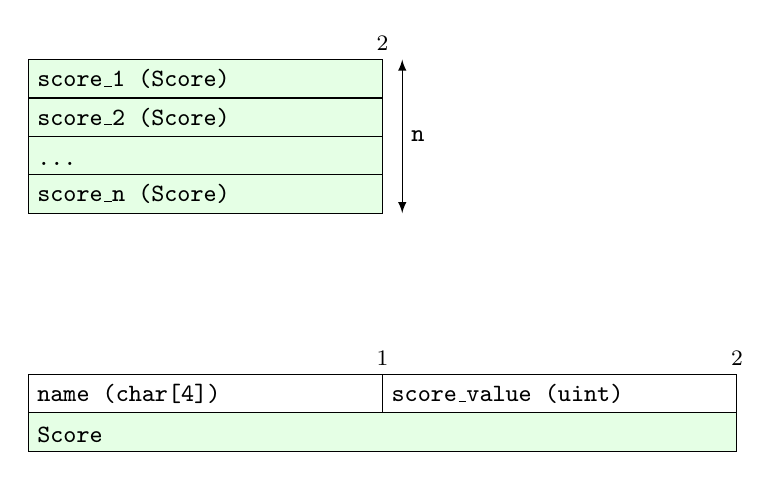
\begin{tikzpicture}
\small
\def\sz{4.5}

\draw[fill=green!10] (0,4) node[anchor=south west]{\texttt{score\_1 (Score)}} rectangle +(\sz,1.5em) node[above]{\footnotesize 2};
\draw[fill=green!10] (0,4cm-1.5em) node[anchor=south west]{\texttt{score\_2 (Score)}} rectangle +(\sz,1.5em);
\draw[fill=green!10] (0,4cm-3em) node[anchor=south west]{\texttt{...}} rectangle +(\sz,1.5em);
\draw[fill=green!10] (0,4cm-4.5em) node[anchor=south west]{\texttt{score\_n (Score)}} rectangle +(\sz,1.5em);

\draw[latex-latex] (\sz cm+.25cm,4cm+1.5em) -- node[right]{\texttt{n}} +(0,-6em);


\draw (0,0) node[anchor=south west]{\texttt{name (char[4])}} rectangle +(\sz,1.5em) node[above]{\footnotesize 1};
\draw (1*\sz,0) node[anchor=south west]{\texttt{score\_value (uint)}} rectangle +(\sz,1.5em) node[above]{\footnotesize 2};
\draw[fill=green!10] (0,-1.5em) node[anchor=south west]{\texttt{Score}} rectangle +(2*\sz,1.5em);
\end{tikzpicture}
\caption{Definition of the file to store scores.}
\label{fig:def:scores}
\end{figure} 

\subsubsection{Data file (\texttt{datafile.h})}

The only function in this module is:\begin{minted}{c}
int datafile_line_field_positions(char* text, unsigned int num_data, char** positions, char** nextstart);
\end{minted}

It splits a given line (starting at \cc{text}) into \textit{fieds} (space separated) and fill \cc{positions} with the starting position of each field. It expects \cc{num_data} fields, otherwise it returns something different from 0. But everything after the \texttt{\#} character is ignored (comment character), so the function may return 1 if this is a line with just a comment (who needs to be skipped). \cc{nextstart} is set to the next line, or \cc{NULL} if \cc{'\0'} is reached.

\subsubsection{Definitions of objects (\texttt{object\_definitions.h})}

Used to define and list the properties of a given type of item or monster. The game engine will use a pointer to refer to those definitions when creating and using an actual item or monster.

\begin{minted}[breaklines]{c}
// items
typedef enum extra_power_t_ {
	EP_NONE,
	EP_ADD_LIFE,
	EP_ADD_EXTRA_LIFE,
	EP_FULL_HEAL,
	EP_NUMBER
} extra_power_t;

typedef struct ItemDef_ {
	unsigned int points_given;
	Sprite* sprite;
	extra_power_t extra_power;
} ItemDef;

ItemDef *item_def_new(unsigned int points_given, extra_power_t extra_power, Sprite *sprite);
void item_def_delete(ItemDef* item);

#define ITEM_WIDTH 32 // [pixels]
#define ITEM_HEIGHT 32 // [pixels]

ItemDef** item_defs_from_file(FILE* f, Image* items_texture, unsigned int* size);

// monsters
enum {
    MA_NORMAL,
    MA_ANGRY,
    MA_CAPTURED,
    MA_NUMBER
};

typedef struct MonsterDef_ {
	Animation* animation[MA_NUMBER];
	unsigned int speed; // number of frames between two movements
} MonsterDef;

MonsterDef* monster_def_new(Animation **sprite_animation, unsigned int speed);
void monster_def_delete(MonsterDef* item);

#define MONSTER_WIDTH 32 // [pixels]
#define MONSTER_HEIGHT 32 // [pixels]
#define MONSTER_FRAMERATE 10 // [frames]

MonsterDef** monster_defs_from_file(FILE* f, Image* items_texture, unsigned int* size);
\end{minted}


The last functions for each structure (\cc{*_defs_from_file()}) loads and return an array of item (monster) definitions (of \cc{size} elements) defined in a text file. There is one item (one monster) per line, defined by the information given in Figure \ref{fig:def:items} (Figure \ref{fig:def:monsters}). The data structure is therefore the one given in Figure \ref{fig:def:tab}, an array of pointers. Note that the code assumes the size of the item and monsters to be always the same, a 32x32 pixels square.

\begin{figure}[!p]
	\centering
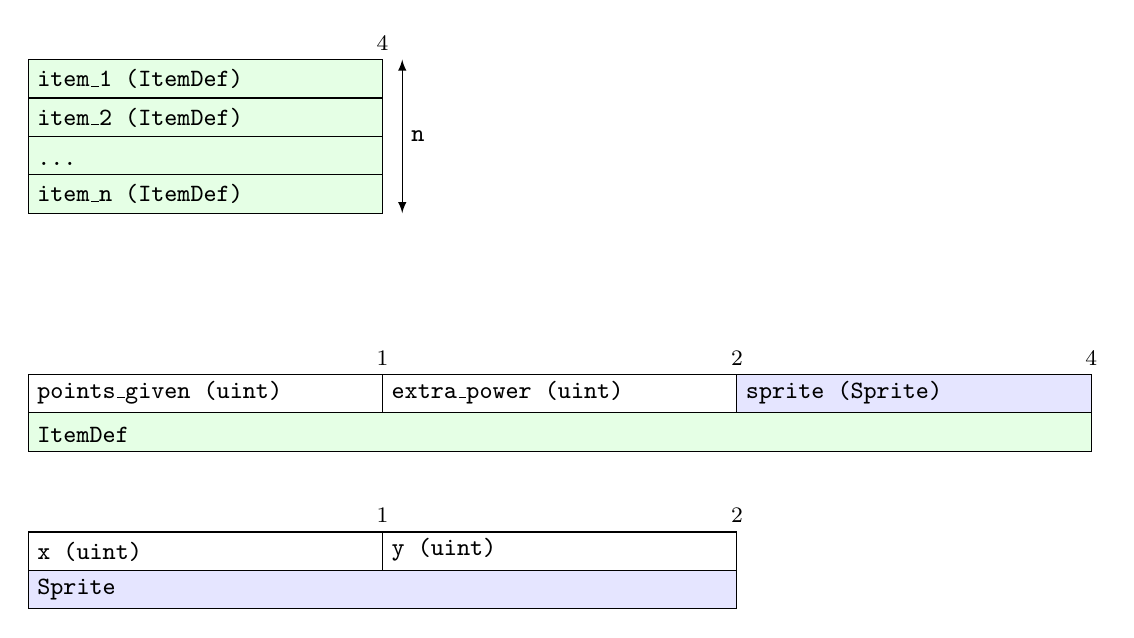
\begin{tikzpicture}
\small
\def\sz{4.5}

\draw[fill=green!10] (0,4) node[anchor=south west]{\texttt{item\_1 (ItemDef)}} rectangle +(\sz,1.5em) node[above]{\footnotesize 4};
\draw[fill=green!10] (0,4cm-1.5em) node[anchor=south west]{\texttt{item\_2 (ItemDef)}} rectangle +(\sz,1.5em);
\draw[fill=green!10] (0,4cm-3em) node[anchor=south west]{\texttt{...}} rectangle +(\sz,1.5em);
\draw[fill=green!10] (0,4cm-4.5em) node[anchor=south west]{\texttt{item\_n (ItemDef)}} rectangle +(\sz,1.5em);

\draw[latex-latex] (\sz cm+.25cm,4cm+1.5em) -- node[right]{\texttt{n}} +(0,-6em);


\draw (0,0) node[anchor=south west]{\texttt{points\_given (uint)}} rectangle +(\sz,1.5em) node[above]{\footnotesize 1};
\draw (1*\sz,0) node[anchor=south west]{\texttt{extra\_power (uint)}} rectangle +(\sz,1.5em) node[above]{\footnotesize 2};
\draw[fill=blue!10]  (2*\sz,0) node[anchor=south west]{\texttt{sprite (Sprite)}} rectangle +(\sz,1.5em) node[above]{\footnotesize 4};
\draw[fill=green!10] (0,-1.5em) node[anchor=south west]{\texttt{ItemDef}} rectangle +(3*\sz,1.5em);

\draw (0,-2) node[anchor=south west]{\texttt{x (uint)}} rectangle +(\sz,1.5em) node[above]{\footnotesize 1};
\draw (\sz,-2) node[anchor=south west]{\texttt{y (uint)}} rectangle +(\sz,1.5em) node[above]{\footnotesize 2};
\draw[fill=blue!10] (0,-2cm-1.5em) node[anchor=south west]{\texttt{Sprite}} rectangle +(2*\sz,1.5em);
\end{tikzpicture}
\caption{Definition of the file to store item definitions. The \texttt{extra\_power} value will be converted to \texttt{extra\_power\_t}.}
\label{fig:def:items}
\end{figure}

\begin{figure}[!p]
	\centering
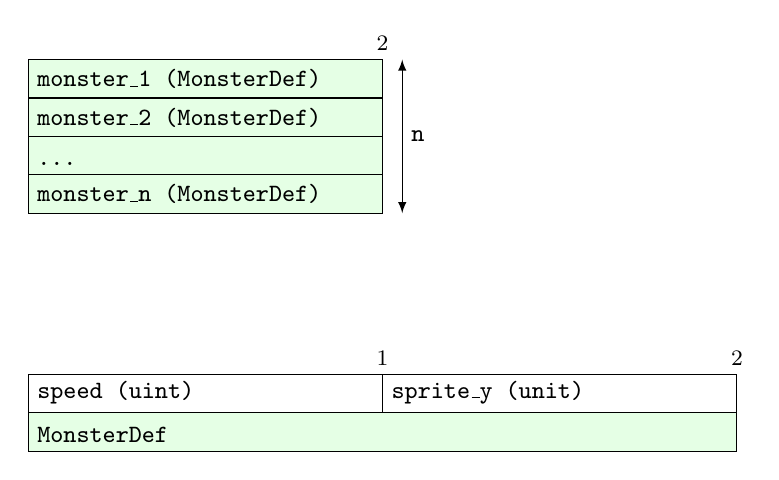
\begin{tikzpicture}
\small
\def\sz{4.5}

\draw[fill=green!10] (0,4) node[anchor=south west]{\texttt{monster\_1 (MonsterDef)}} rectangle +(\sz,1.5em) node[above]{\footnotesize 2};
\draw[fill=green!10] (0,4cm-1.5em) node[anchor=south west]{\texttt{monster\_2 (MonsterDef)}} rectangle +(\sz,1.5em);
\draw[fill=green!10] (0,4cm-3em) node[anchor=south west]{\texttt{...}} rectangle +(\sz,1.5em);
\draw[fill=green!10] (0,4cm-4.5em) node[anchor=south west]{\texttt{monster\_n (MonsterDef)}} rectangle +(\sz,1.5em);

\draw[latex-latex] (\sz cm+.25cm,4cm+1.5em) -- node[right]{\texttt{n}} +(0,-6em);


\draw[] (0,0) node[anchor=south west]{\texttt{speed (uint)}} rectangle +(\sz,1.5em) node[above]{\footnotesize 1};
\draw[]  (1*\sz,0) node[anchor=south west]{\texttt{sprite\_y (unit)}} rectangle +(\sz,1.5em) node[above]{\footnotesize 2};
\draw[fill=green!10] (0,-1.5em) node[anchor=south west]{\texttt{MonsterDef}} rectangle +(2*\sz,1.5em);
\end{tikzpicture}
\caption{Definition of the file to store monster definitions. Since it is assumed that all the sprites of a monster are on the same line, only \texttt{srpite\_y} (the $y$ position of the sprite) is required.}
\label{fig:def:monsters}
\end{figure}

\begin{figure}[!h]
\centering
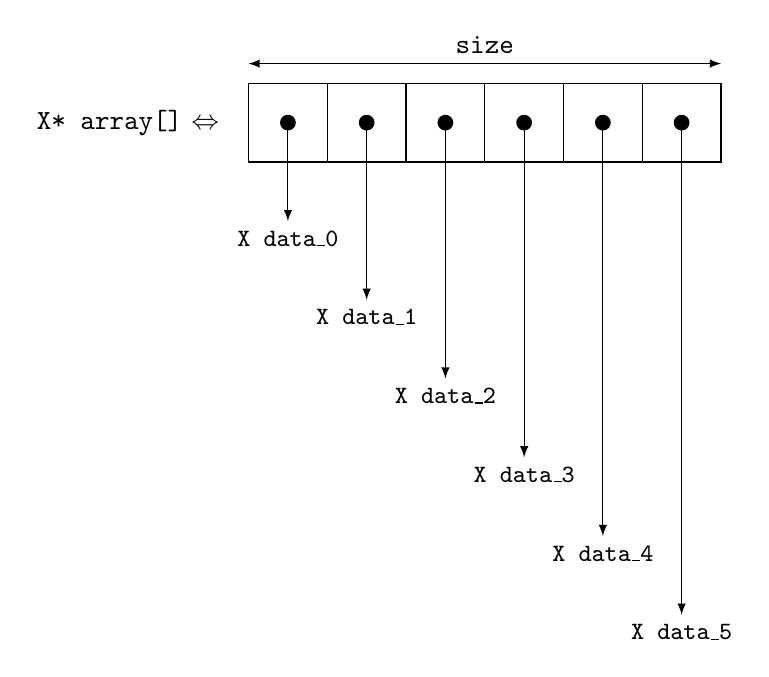
\begin{tikzpicture}
\foreach\i in {0,1,2,3,4,5} {
\draw (\i,0) rectangle +(1,1);
\fill (\i+.5,.5) circle (.1cm);
\draw[-latex] (\i+.5,.5) -- +(0,-1-\i.25) node[below]{\small \texttt{X data\_\i}};
}

\draw (-.25,.5) node[left]{\texttt{X* array[]} $\Leftrightarrow$ };

\draw[latex-latex] (.0,1.25) -- node[midway,above]{\texttt{size}} +(6,0);
\end{tikzpicture}
\caption{Data structure of an array of size \cc{size} (here, 5) of pointers to a structure \cc{X}.}
\label{fig:def:tab}
\end{figure}

Note that the choice to use arrays here is not innocent, since those definitions will be called via their positions in the table (corresponding to their positions in the file) in the levels (see below).

\subsubsection{Levels (\texttt{levels.h})}

A level (NULL terminated chained list) contains the map, which is stored as a 1-D array.

\begin{minted}[breaklines]{c}
#define TILE_WIDTH 16 // [pixels]
#define TILE_HEIGHT 16 // [pixels]
#define MAP_WIDTH 32 // [cases]
#define MAP_HEIGHT 24 // [cases]

typedef struct Position_ {
    unsigned int x;
    unsigned int y;
}  Position;

int position_index(Position pos);

typedef struct Level_ {
    bool map[MAP_HEIGHT * MAP_WIDTH];
    Position bubble_endpoint;
    Sprite* fill_tile;
    unsigned int num_monsters;
    MonsterDef** monsters; // dynamically allocated
    Position* monster_positions; // dynamically allocated
    struct Level_* next; // NULL terminated
} Level;

Level* level_new(bool *map, Position bubble_endpoint, Sprite *fill_tile, unsigned int num_monsters, MonsterDef **monsters, Position *monster_positions);
void level_delete(Level* level);

Level *level_new_from_string(char *buffer, int *position, Image *image_level, MonsterDef **base_monster_defs,int num_monster_defs);
Level *levels_new_from_file(FILE *f, Image *image_level, MonsterDef **base_monster_defs, int num_monster_defs,nsigned int *num_levels);

void blit_level(Level *level, int y_shift);
\end{minted} 

The level also contains the tile used for the filled element in the map, a list of the monster with their initial position, and the final position of the bubble.

The \cc{level_new_from_file()} function create the level from a \textbf{portion} of a text file, for which the definition is pictured in Figure \ref{fig:def:level}. At the end of this function, the file cursor is set to the next level: since the number of lines is known when the header is read (\text{1 + \cc{num_monster} + 24}), it is actually possible to store all levels in a file. The function \cc{levels_new_from_file()} read the whole file (by calling \cc{level_new_from_string()} repetitively until \cc{EOF}) and create the chained list. 

\begin{sidewaysfigure}
\centering
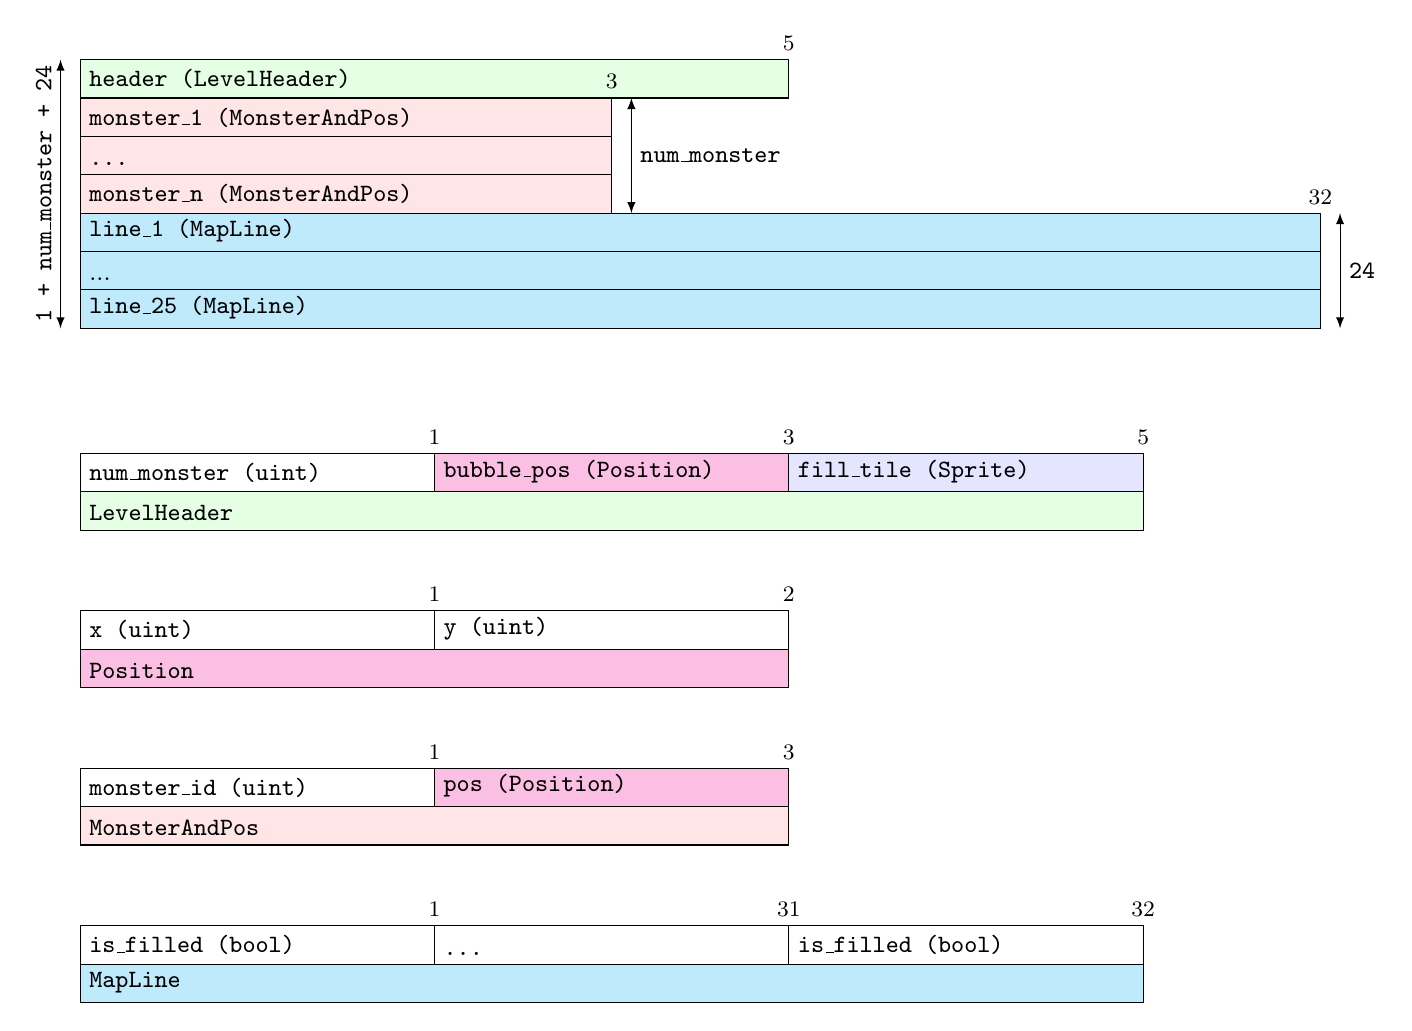
\begin{tikzpicture}
\small
\def\sz{4.5}

\draw[fill=green!10] (0,4) node[anchor=south west]{\texttt{header (LevelHeader)}} rectangle +(2*\sz,1.5em) node[above]{\footnotesize 5};
\draw[fill=red!10] (0,4cm-1.5em) node[anchor=south west]{\texttt{monster\_1 (MonsterAndPos)}} rectangle +(1.5*\sz,1.5em)node[above]{\footnotesize 3};
\draw[fill=red!10] (0,4cm-3em) node[anchor=south west]{\texttt{...}} rectangle +(1.5*\sz,1.5em);
\draw[fill=red!10] (0,4cm-4.5em) node[anchor=south west]{\texttt{monster\_n (MonsterAndPos)}} rectangle +(1.5*\sz,1.5em);
\draw[fill=cyan!25] (0,4cm-6em) node[anchor=south west]{\texttt{line\_1 (MapLine)}} rectangle +(3.5*\sz,1.5em)node[above]{\footnotesize 32};
\draw[fill=cyan!25] (0,4cm-7.5em) node[anchor=south west]{...} rectangle +(3.5*\sz,1.5em);
\draw[fill=cyan!25] (0,4cm-9em) node[anchor=south west]{\texttt{line\_25 (MapLine)}} rectangle +(3.5*\sz,1.5em);

\draw[latex-latex] (1.5*\sz cm+.25cm,4cm) -- node[right]{\texttt{num\_monster}} +(0,-4.5em);
\draw[latex-latex] (3.5*\sz cm+.25cm,4cm-4.5em) -- node[right]{\texttt{24}} +(0,-4.5em);
\draw[latex-latex] (-.25cm,4cm+1.5em) -- node[above,rotate=90]{\texttt{1 + num\_monster + 24}} +(0,-10.5em);


\draw (0,-1) node[anchor=south west]{\texttt{num\_monster (uint)}} rectangle +(\sz,1.5em) node[above]{\footnotesize 1};
\draw[fill=magenta!25] (1*\sz,-1) node[anchor=south west]{\texttt{bubble\_pos (Position)}} rectangle +(\sz,1.5em) node[above]{\footnotesize 3};
\draw[fill=blue!10]  (2*\sz,-1) node[anchor=south west]{\texttt{fill\_tile (Sprite)}} rectangle +(\sz,1.5em) node[above]{\footnotesize 5};
\draw[fill=green!10] (0,-1cm-1.5em) node[anchor=south west]{\texttt{LevelHeader}} rectangle +(3*\sz,1.5em);

\draw (0,-3) node[anchor=south west]{\texttt{x (uint)}} rectangle +(\sz,1.5em) node[above]{\footnotesize 1};
\draw (\sz,-3) node[anchor=south west]{\texttt{y (uint)}} rectangle +(\sz,1.5em) node[above]{\footnotesize 2};
\draw[fill=magenta!25] (0,-3cm-1.5em) node[anchor=south west]{\texttt{Position}} rectangle +(2*\sz,1.5em);

\draw (0,-5) node[anchor=south west]{\texttt{monster\_id (uint)}} rectangle +(\sz,1.5em) node[above]{\footnotesize 1};
\draw[fill=magenta!25] (\sz,-5) node[anchor=south west]{\texttt{pos (Position)}} rectangle +(\sz,1.5em) node[above]{\footnotesize 3};
\draw[fill=red!10] (0,-5cm-1.5em) node[anchor=south west]{\texttt{MonsterAndPos}} rectangle +(2*\sz,1.5em);

\draw (0,-7) node[anchor=south west]{\texttt{is\_filled (bool)}} rectangle +(\sz,1.5em) node[above]{\footnotesize 1};
\draw(\sz,-7) node[anchor=south west]{\texttt{...}} rectangle +(\sz,1.5em) node[above]{\footnotesize 31};
\draw(2*\sz,-7) node[anchor=south west]{\texttt{is\_filled (bool)}} rectangle +(\sz,1.5em) node[above]{\footnotesize 32};
\draw[fill=cyan!25] (0,-7cm-1.5em) node[anchor=south west]{\texttt{MapLine}} rectangle +(3*\sz,1.5em);
\end{tikzpicture}
\caption{Definition of the file to store a level. The \texttt{num\_monster} value (in the \texttt{LevelHeader} structure) is used to determine how many monster lines (\texttt{MonsterAndPos} structures) there will be. The \texttt{monster\_id} value (in \texttt{MonsterAndPos}) refers to the line in the monster definition file. The \texttt{MapLine} structure is repeated 24 times and contains 32 boolean to indicate whether the square is filled or not (since a map is 32$\times$24 squares). The \texttt{Sprite} structure (blue) is the same as in Figure \ref{fig:def:items}.}
\label{fig:def:level}
\end{sidewaysfigure} 

The \cc{Position} structure represents a position in terms of the number of cases. But to get better (and smoother) movements, it is interesting to have a more general structure to deal with position in the level: the \cc{LevelObject} structure.

\begin{minted}[breaklines]{c}
typedef struct LevelObject_ {
    Position position;
    int width;
    int height;

    bool move_forward;
    Counter* counter_x;
    Counter* counter_y;
    Counter* counter_jump;
    Counter* counter_chase;    
    bool is_falling;
    bool falling_from_above;
    Position target_position;
} LevelObject;

LevelObject *level_object_new(Position position, int width, int height);
void level_object_delete(LevelObject *map_object);

LevelObject* level_object_copy(LevelObject *src);

bool level_object_test_left(LevelObject *representation, Level *level);
bool level_object_test_right(LevelObject *representation, Level *level);
bool level_object_test_up(LevelObject *representation, Level *level);
bool level_object_test_down(LevelObject *representation, Level *level);

bool level_object_can_move(LevelObject *obj);
bool level_object_can_jump(LevelObject *obj);

bool level_object_move_left(LevelObject *representation, Level *level);
bool level_object_move_right(LevelObject *representation, Level *level);
bool level_object_jump(LevelObject *representation, Level *level, int jump);
void level_object_adjust(LevelObject *representation, Level *level);

void level_object_chase(LevelObject *moving, LevelObject *target, Level *level, int speed);

#define FALLING_FROM (MAP_HEIGHT + 2) // cases

void level_object_set_falling_from_above(LevelObject *obj, Position target);
\end{minted}

This object is the representation of any object that can appear on the map. It contains the position, but the ``real" position on the level is modulated by \cc{counter_x} and \cc{counter_y}. In pseudo-code,\begin{minted}{c}
float real_x = x + (float) (move_forward ? -1 : 1) * counter_x / MOVE_EVERY;
float real_y = y + (float) (is_falling ? 1 : -1) * counter_y / MOVE_EVERY;
\end{minted}

If the object is moved, \cc{x} and \cc{y} are modified accordingly. But with the helps of the counter, which delays the movement, the object will appear to move to the new position in a few frames, not instantaneously. Other counters also help in the case of jumping (to know how much it must jump, with \cc{counter_jump}) or in the case of chasing (an object can move in the direction of another, but change direction every few frame, with \cc{counter_chase}).

The \cc{level_object_adjust()} function ``adjust" the object: it ticks the counters, and check if the object should start (empty tile below) or stop (solid tile below) to fall. Note that an object can start by \textit{falling from above}, which simulate the fact that some object fall from the top of the screen to a given target position (using the \cc{level_object_set_falling_from_above()} function sets the corresponding variables).

This structure is therefore used to do collisions tests with the map, with the different \cc{level_object_test_*()} functions, and movements with the different \cc{level_object_move_*()} and \cc{level_object_jump()} functions (which test if the movement is possible before setting the position and the counters, basically). The \cc{level_object_can_*()} function checks if a movement is possible (only if the corresponding counter is stopped).

The chasing algorithm (exploited by the monsters, see below) is fairly simple:\begin{enumerate}
\item If the object is above the target, it will try to find a hole in the floor (the closest one), and jump into it to get closer ;
\item If the object is below the target, it will try to jump ;
\item If jumping is not possible, the object will go left or right, depending on the $x$ value of the target.
\end{enumerate}
This algorithm actually works quite well on many of the map of the original game (and all of the current implementation), but it wouldn't work if both objects have the same $y$ but are separated by a wall. If so, the object should know where to jump to get closer to the target. Note that the \cc{speed} parameter controls the delay between to chasing events, and therefore controls at which speed an object gets closer to another. It is therefore expected that monster with more speed (see above in \cc{MonsterDefinition}) chase less than a monster with lower speed (which are therefore more difficult to catch).

Finally, it is interesting to check whether two objects are in the collision. To do so, an \textit{effective position}, computed as \cc{real_x} and \cc{real_y} given above, is needed:
\begin{minted}{c}
#define CONTACT_DISTANCE 4

typedef struct EffectivePosition_ {
	float x;
	float y;
} EffectivePosition;

EffectivePosition level_object_to_effective_position(LevelObject *mobj);
bool level_object_in_collision(LevelObject *a, LevelObject *b);
\end{minted}

The \cc{level_object_in_collision()} uses the distance between the two objects, computed as $\sqrt{(x_B-x_A)^+(y_B-y_A)^2}$. For the objects to be in collision, this distance should be lower than the square root of \cc{CONTACT_DISTANCE} (to avoid the useless computation of a square root, all is squared).

\subsubsection{Game objects (\texttt{game\_objects.h})}

Now that the level is defined, the different objects may be as well. Items and monsters also have a pointer to their definition (to know the sprites, etc.). Finally, they are all \cc{NULL} terminated chained lists (except the dragon). Lets start with monsters and items:

\begin{minted}{c}
#define MONSTER_WIDTH 32 // [pixels]
#define MONSTER_HEIGHT 32 // [pixels]
#define MONSTER_FRAMERATE 10 // [frames]
#define MONSTER_JUMP 6 // [case] (height of jump)

typedef struct Monster_ {
    LevelObject* map_object;
    MonsterDef* definition;
    Animation* animation[MA_NUMBER];
    bool angry;
    bool in_bubble;
    struct Monster_* next;
} Monster;

Monster* monster_new(LevelObject* map_object, MonsterDef* definition);
void monster_delete(Monster* monster);

Monster* monsters_new_from_level(Level* level);
Monster* monster_kill(Monster* list, Monster* monster);
void monsters_adjust(Monster* list, Level* level, LevelObject* target);
bool test_collide_other_monsters(Monster* moving, Monster* list, LevelObject* npos);
void blit_monster(Monster *monster, bool frozen);

#define ITEM_JUMP 8 // [cases]
#define ITEM_INVULNERABILITY 30 // [frames]

typedef struct Item_ {
    LevelObject* map_object;
    ItemDef* definition;
    bool go_right;
    Counter* counter_invulnerability;
    struct Item_* next;
} Item;

Item* item_new(LevelObject* map_object, ItemDef* definition);
void item_delete(Item* item);

Item *item_create(LevelObject *position, Item *list, ItemDef **definitions, int num_item_definitions, Level *level, float ratio_time_left);
void items_adjust(Item* list, Level* level);
void blit_item(Item* item);
\end{minted}

Concerning the different structure, the \cc{Item} contains a \cc{go_right} parameter. Indeed, when a bubble is busted, the item \textit{jumps out} the bubble. This parameter determine the direction of the jump (which is used by \cc{items_adjust()}). There is also a \cc{vulnerability_counter}, which is an amount of time when the item cannot be consumed.

The \cc{item_create()} function is different from the \cc{item_new()} function, since it adds the item to a list of existing items (the \cc{list} parameter) and returns the updated list (note that if \cc{list} is \cc{NULL}, a new list is created). This function also pick up an item to create in the list of definition. Since this list is expected to be sorted in rarity of the item (most common and low point items first), the function picks the items depending on \cc{ratio_time_left} (the largest the value, the lower the value of the item). But in order to avoid a minimum getting the same object when two bubbles are burst by the dragon at the same time, a small amount of random is added.

Concerning \cc{Monster}, the \cc{angry} parameter is a parameter used to determine if the monster is angry: a monster is angry when he was in a bubble and escape because the bubble burst on its own (see below). If this parameter is set to \cc{true}, the monster move faster. Finally, the \cc{in_bubble} parameter is used to determine if the monster is into a bubble (if so, it does not draw on the screen). The \cc{monster_adjust()} function set the monster chasing the dragon, and avoid a collision between monsters (otherwise monsters end up all in the same position and walk together so that it is difficult to distinguish them).

\begin{minted}{c}
typedef struct Bubble_ {
    LevelObject* map_object;
    Animation* animation;

    Monster* captured; // NULL in the beginning

    Counter* counter_momentum; // counter until it moves on its own
    Counter* counter_time_left; // counter until it auto-burst
    EffectivePosition force;
    struct Bubble_* next; // NULL terminated
} Bubble;

#define BUBBLE_WIDTH 32 // [pixels]
#define BUBBLE_HEIGHT 32 // [pixels]
#define BUBBLE_FRAMERATE 10 // [frames]

#define BUBBLE_MOMENTUM 10 // [frames]
#define BUBBLE_TIME 600 // [frames]

#define BUBBLE_X 0 // [pixels]
#define BUBBLE_Y 32 // [pixels]

#define BUBBLE_K_POS .5f
#define BUBBLE_K_INTER 1.f
#define BUBBLE_REQ_POS .5f
#define BUBBLE_REQ_INTER 3.f
#define BUBBLE_MIN_FORCES 5.f // avoid shakiness of the bubbles

Bubble *bubble_new(LevelObject *map_object, Image *texture, bool go_right);
void bubble_delete(Bubble* bubble);

Bubble* bubbles_adjust(Bubble *bubble_list, Level *level, Position final_position);
Bubble *bubble_burst(Bubble *bubble_list, Bubble *bubble, bool free_monster);
\end{minted}

The movement of a bubble is very specific: it starts by going in the direction it has been blown, until it loses its \textit{momentum}. When it does, all the bubbles end up in about the same position in the level. Bubbles burst on their own after a time, freeing the monster that they contain if it was the case. The \cc{Bubble} structure has a \cc{counter_momentum} parameter, that if 0, the bubble stops to go in the initial direction (indicated by \cc{go_right} in \cc{LevelObject}) and starts to go in the direction of \cc{bubble_endpoint} (in \cc{Level}, see above). \cc{counter_time_left} is another counter. If its value becomes 0, the bubble burst and release the monster (stored in \cc{captured}) that it eventually contains (which becomes angry). All of that is done by the \cc{bubbles_adjust()} functions, which also take care that the bubble does not end up in the same position by exploiting \cc{force} (see below).

To do so, the code adds virtual springs\footnote{This kind of approach comes from my physic lectures.} Between the bubble and the final position, and between the bubbles, so that bubbles are attracted by the final position and other bubbles if they are at long distances (the spring is elongated) and repulsed at short distances (the spring is compressed). According to the Hooke's law \cite{hooke}, the potential energy of a spring for which ends are $a$ and $b$ is given by\begin{equation}
U_{ab} = k\,(||\vec{p}_a-\vec{p}_b||-r_{ab})^2,
\end{equation}
where $\vec{p}_X$ is the position of $X$, $k$ is the force constant (the difficulty to elongate the spring) and $r_{ab}$ is the resting distance (the ideal position). The force, on one end on the spring ($b$) due to the other side ($a$) is given by the gradient (the derivative) of the potential, so\begin{equation}
\vec{F}_{ab}  = - \vec{\nabla} U_{ab} =  -2\,k\,(||\vec{p}_a-\vec{p}_b||-r_{ab})\,\frac{\vec{p}_b-\vec{p}_a}{||\vec{p_b}-\vec{p}_A||},
\end{equation}
where the force is therefore a vector. The force on a given bubble is the force of all spring acting on it, $\vec{F}_a = \sum_{b\neq a} \vec{F}_{ab}$, and this forces tends to zero when an equilibrium situation is reached (corresponding to a minimum in the energy of the system). Also, solving Newtown equations of motion gives the following relation\begin{equation}
\vec{p}_A(t+\Delta{t}) = \vec{p}_A(t) + \Delta{t}^2\,\frac{\vec{F}_A}{m},\label{eq:1}
\end{equation}
so the new position of the bubble after a time $\Delta{t}$, $\vec{p}_A(t+\Delta{t})$ proportional to the old position, $\vec{p}_A(t)$ plus $\vec{F}_A$ (setting the mass of the body, $m$, to 1 and $\Delta{t}$ to 1). This last formula is coded into \cc{bubble_adjust()}\footnote{To be precise, in \cc{force_expr()} in \texttt{game\_objects.c}, used by \cc{bubble_update_force()}, which computes $\vec{F}_{a}$ for each bubble and store it into \cc{force}.}, which uses the total force to decide the direction of the next movement (up, down, left or right). The different forces constants and equilibrium distances are given by \cc{BUBBLE_K_*} and \cc{BUBBLE_REQ_*} (adjusted by trial and error). Below a minimal force (\cc{BUBBLE_MIN_FORCES}, also adjusted by trial and errors), the bubble is not moved (and is said to be in an equilibrium position). This approach, although a bit overkill, works quite well, as pictured in Figure \ref{fig:def:bubs}.

\begin{figure}[!h]
\centering
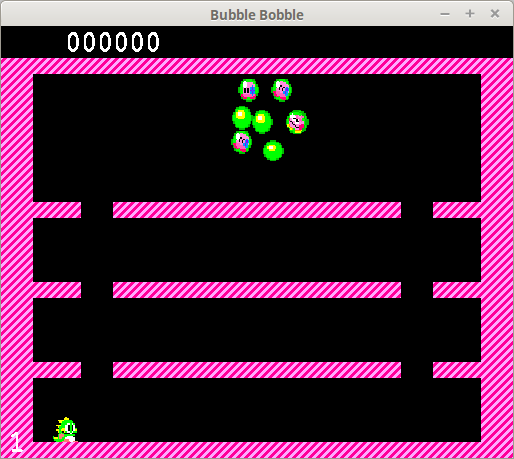
\includegraphics[width=.6\linewidth]{i/screen6}
\caption{Illustration of the implementation of Eq.~\ref{eq:1} to control the bubbles.}
\label{fig:def:bubs}
\end{figure}

Finally, a structure to represent the dragons is also needed:

\begin{minted}{c}
enum {
    DA_NORMAL,
    DA_MOVE,
    DA_BLOW,
    DA_HIT,
    DA_INVICIBLE,
    DA_NUMBER
};

#define DRAGON_WIDTH 32 // [pixels]
#define DRAGON_HEIGHT 32 // [pixels]
#define DRAGON_FRAMERATE 10 // [frames]

#define DRAGON_LIFE 3
#define DRAGON_JUMP 6 // [cases] of jump
#define DRAGON_INVINCIBILITY 120 // [frames]
#define DRAGON_HIT 60 // [frames]
#define DRAGON_BLOW 4 // [frames]

typedef struct Dragon_ {
    LevelObject* map_object;
    Position respawn_position; // to respawn
    Animation* animations[DA_NUMBER]; // animations
    unsigned int score;
    int life; // 3 at the beginning
    int max_life; // 3 at the beginning

    bool hit; // hit!
    bool invincible; // when just killed
    Counter* counter_hit;
    Counter* counter_blow;
    Counter* counter_invincible;
} Dragon;

Dragon *dragon_new(LevelObject *map_object, Animation **animation);
void dragon_delete(Dragon* dragon);
void blit_dragon(Dragon *dragon, bool frozen, int shift_y);

void dragon_adjust(Dragon *dragon, Level *level);
Bubble* dragon_blow(Dragon* dragon, Bubble* bubble_list, Image* texture);
Item* dragon_consume_item(Dragon* dragon, Item* list, Item* item);

#define POSITION_BUB (Position) {3, 1}
#define BUB_Y 0

Dragon* create_bub(Image* texture, int y); // explicitly create Bub!
\end{minted}

It is the dragon object which contains the score (since in a two-player version, each player would control its dragon, with a personal score). The dragon has a given \cc{life}, and a \cc{max_life}, so that the item cannot heal the dragon more than the maximum. There are 3 counters: \cc{counter_hit}, which display the \cc{DA_HIT} animation when hit by a monster (\cc{hit} is set to true), during a few frames before actually get killed, respawn at \cc{respawn_position} and get invincible (\cc{invincible} is set to true), during the time controlled by \cc{counter_invincible}. The \cc{counter_blow} display the \cc{DA_BLOW} animation during a few frames when blowing a bubble. Those counters are managed by \cc{dragon_adjust()} (which move the dragon to its respawn position when dead and set it invincible).

The \cc{dragon_blow()} and \cc{dragon_consume_item()} functions respectively create a bubble and add it to the list of bubbles, and remove an item from the list (and get the point and apply its eventual extra power, see above). Since those are NULL terminated lists, the first function may receive NULL as an argument (if the list of bubbles is empty) and the latter may return NULL (if there is no more item left after consuming the last one).

\subsubsection{The base game structure (\texttt{game\_base.h})}

\label{p:ekey}Due to the way that GLUT works \cite{freeglut},  it is required to know whether a keyboard key is pressed or not in the main game loop (see below). To do so, some defines are required :\begin{minted}{c}
#define FRAMES_BETWEEN_KEY_REPEAT_IN_SCREEENS 8 // [frames]
#define FRAMES_BETWEEN_KEY_REPEAT_IN_GAME 4 // [frames]

enum {
    E_NONE,
    E_LEFT,
    E_RIGHT,
    E_UP,
    E_DOWN,
    E_ACTION_1, // i.e. "jump"
    E_ACTION_2, // i.e. "blow"
    E_FREEZE,
    E_SHOW_SCORE,
    E_SHOW_CONTROLS,
    E_QUIT,
    E_SIZE
};

void keys_init(Game* game);
void keys_delete(Game* game);

void keys_update_interval(Game *game);
void keys_reset(Game *game);
void key_down(Game *game, int key);
void key_up(Game *game, int key)
bool key_fired(Game* game, int key);
\end{minted}

In the \cc{Game} structure (see below), there will be two arrays:\begin{enumerate}
\item A boolean \cc{key_pressed[E_SIZE]} array. Values of this array are set to \cc{true} when a keyboard key is pressed, and \cc{false} when released (using \cc {key_down()} and \cc{key_up()} to register the pressed keys). \cc{keys_reset()} simply set the whole array to \cc{false}.
\item A counter \cc{key_counters[E_SIZE]} array, which will be started when a key is pressed, and for which the value will increase at each frame while the key is pressed (with \cc{keys_update_interval()}). The goal is to keep track of the time since a key has been pressed, and eventually repeat the event, every time the counter reaches its maximum (\cc{FRAMES_BETWEEN_KEY_REPEAT_IN_*}, depending on which state the program is, see below). The \cc{key_fired()} function is used to determine whether both conditions are satisfied.
\end{enumerate}

The \cc{Game} structure will contain everything needed to run the game, and will be instanced once, as one of the (few) global variables.

\begin{minted}{c}
enum {
    SCREEN_WELCOME,
    SCREEN_INSTRUCTIONS,
    SCREEN_GAME_OVER,
    SCREEN_WIN,
    SCREEN_SCORE,
    SCREEN_NUMBER
};

#define GAME_ELEMENT_WIDTH 32 // [pixels]
#define GAME_ELEMENT_HEIGHT 32 // [pixels]

#define NEXT_LEVEL_TRANSITION 120 // [frames]
#define UNTIL_NEXT_LEVEL 600 // [frames]
#define FREEZE_EVERY 30 // [frames]
#define MAX_LEVEL_TIME (30 * 60) // [frames]

enum {
    GE_ARROW,
    GE_NUMBER
};

typedef struct Game_ {
    bool paused;
    bool main_started;
    bool freeze;

    // Image
    Image* texture_game;
    Image* texture_items;
    Image* texture_monsters;
    Image* texture_levels;
    Image* texture_dragons;
    Image* texture_screens;
    Image* texture_font;

    int current_screen;
    Sprite* screens[SCREEN_NUMBER];
    Sprite* game_elements[GE_NUMBER];
    Font* font;
    
    // scores
    Score* scores_list;

    // definitions
    ItemDef** definition_items;
    unsigned int num_items_defined;
    MonsterDef** definition_monsters;
    unsigned int num_monsters_defined;

    // levels
    Level* levels;
    Level* current_level;
    Level* previous_level;
    Level* starting_level;
    unsigned int num_levels;

    Counter* counter_next_level;
    Counter* counter_end_this_level;
    Counter* counter_start_level;

    // dragons & monsters & bubbles & items
    Dragon* bub;
    Monster* monster_list;
    Bubble* bubble_list;
    Item* item_list;

    // keys
    bool key_pressed[E_SIZE];
    Counter* key_counters[E_SIZE];
    int key_interval;
} Game;
\end{minted}

There is a large part of the structure to store the different textures and sprites, and key management as mentioned above. There is also a space for the definitions (see above) and the actual levels (with a pointer to the previous and next level), dragon, items, monster and bubbles (see above). There is also some counters: \cc{counter_next_level}, which is useful for the transition between the levels (the previous level and the next level slides up), \cc{counter_end_this_level}, which is activated when the last monster is killed (and delay the time when the game will automatically go to the next level) and \cc{counter_start_level}, which keeps track of the time since the beginning of the level: if the time is too long, the game sends a monster after the player.

I will make a difference between the \textit{main} game (Bub moving, blowing bubbles, etc.) and the screens. To ease that the structure ends by 3 booleans:\begin{itemize}
\item \cc{paused}: true when a screen is active: the \textit{main} game is paused and the screen is drawn instead.
\item \cc{main_started}: true when the \textit{main} game is launched (it is not the case when the program starts). It is useful to know whether to go back to the game or the welcome screen from other screens.
\item \cc{freeze}: used for the actual pause, when nothing moves.
\end{itemize}

\subsubsection{Screens (\texttt{game\_screens.h})}

\begin{minted}{c}
void game_set_screen(Game* game, int screen);

void game_simple_screen_input_management(Game *game, bool return_to_game);
void game_simple_screen_draw(Game *game);


#define WS_BASE 182 // [pixels]
#define WS_SHIFT 38 // [pixels]

void game_welcome_screen_input_management(Game *game);
void game_welcome_screen_draw(Game *game);


#define WL_BASE_X (WINDOW_WIDTH / 2)
#define WL_BASE_Y (WINDOW_HEIGHT / 2)
#define WL_FRAMERATE 30 // [frames]

void game_win_loose_screen_input_management(Game *game);
void game_win_loose_screen_draw(Game *game);

#define SCORE_SHIFT 2 // [frames]

void game_score_screen_draw(Game *game);
\end{minted}

The first function, \cc{game_set_screen()} set the \cc{current_screen} and \cc{paused} variables in the \cc{Game} structure. Then, there are two functions for each screen, first the function of the type \cc{game_*_screen_input_management()} one, which takes a look at which key is active with \cc{key_fired()} and acts accordingly, and \cc{game_*_screen_draw()} type which draws the screen (usually an image [welcome and instruction screen] but also text with \cc{blit_font()} [win and loose screen]).

\subsubsection{\textit{Main} game (\texttt{game\_main.h})}

The most important part, where everything comes into play:\begin{minted}{c}
#define BLOW_EVERY 60 // [frames]

void game_main_start(Game *game);
void game_next_level(Game *game);
void game_setup_current_level(Game *game);

void game_main_input_management(Game *game);
void game_main_update_states(Game *game);
void game_main_draw(Game *game);
\end{minted}

The structure is similar to the screens, since there is one function to deal with inputs (\cc{game_main_input_management()}) and one to draw the result (\cc{game_main_draw()}). The next function \cc{game_main_update_state()} is more interesting, since that is where all the magic happens:\begin{enumerate}
\item Test if the level should not change, either because there is no more item to collect or because \cc{counter_next_level} reaches its maximum. If it is the case, \cc{game_next_level()} is called.
\item Check if the player is still alive (\cc{life >= 0}). If not, \cc{game_set_screen()} is called to set \cc{SCREEN_GAME_OVER}.
\item Call the \cc{*_adjust()} type functions to tick all internal counters. This is where a monster could escape a bubble (because \cc{counter_time_left} reaches its maximum, and by calling \cc{bubble_burst()} with the \cc{free} function parameter set to \cc{true}). It is also where the dragon eventually get killed (if \cc{counter_hit} reaches its maximum) and the monster chose their direction (with \cc{map_object_chase()}).
\item If \cc{counter_start_level} reaches its maximum, an extra monster is sent after the player and the counter is reset.
\item Test collision between items and bubbles and use \cc{dragon_consume()} if any (update the items list).
\item Test collision between bubbles and dragons, and use \cc{bubble_burst()} if any (with the \cc{free} function parameter set to \cc{false}, update the bubbles list).
\item Check collision between monsters and the dragon (set \cc{hit} to \cc{true} and starts \cc{counter_hit} if any) and collision between monsters and bubbles (set \cc{in_bubble} and \cc{captured} if any).
\end{enumerate}
Note that \cc{game_next_level()} simply set up the \cc{current_level}, \cc{previous_level} and \cc{next_level} pointer, and starts the \cc{counter_next_level} in order for \cc{game_main_draw()} to draw the transition between the two levels. When this is done, \cc{game_setup_current_level()} is called, which populate the list of monsters, clear the list of bubbles and items and restarts \cc{counter_start_level}.

\subsubsection{Top level functions: the game (\texttt{game.h})}

This contains all the callbacks required to interface the code to GLUT:\begin{minted}{c}
#define TEXTURE_ITEMS "assets/items.ppm"
#define TEXTURE_MONSTERS "assets/monsters.ppm"
#define TEXTURE_LEVELS "assets/levels.ppm"
#define TEXTURE_DRAGONS "assets/dragons.ppm"
#define TEXTURE_SCREENS "assets/screens.ppm"
#define TEXTURE_GAME "assets/game.ppm"
#define TEXTURE_FONT "assets/font.ppm"

#define DEFINITION_ITEMS "data/items.txt"
#define DEFINITION_MONSTERS "data/monsters.txt"

#define FILE_LEVELS "data/levels.txt"
#define FILE_SCORES "data/scores.txt"

void game_special_key_down(int key, int x, int y);
void game_special_key_up(int key, int x, int y);
void game_key_down(unsigned char key, int x, int y);
void game_key_up(unsigned char key, int x, int y);

void game_init();
void game_loop();
void game_quit();
\end{minted}

In the \cc{game.c} file, a global \cc{Game* game} variable is defined, and will be used by all the function defined here. The resources defined in the begining (image and data files) are used by \cc{game_init()} to create and setup the \cc{game} structure. This structure is correctly dealoacted at the end of the program by \cc{game_quit()}, using the \cc{atexit()} standard function \cite{cppref}.

The keyboard functions are linked to their GLUT counterparts, \begin{minted}{c}
glutKeyboardFunc(game_key_down);
glutKeyboardUpFunc(game_key_up);
glutSpecialFunc(game_special_key_down);
glutSpecialUpFunc(game_special_key_up);
\end{minted}
and translate the GLUT key code into a internal \cc{E_*} action code (defined in \texttt{game\_base.h} see page \pageref{p:ekey}). They call the \cc{key_down()} and \cc{key_up()} functions defined above to set the corresponding variables in the \cc{game} structure.

The \cc{game_loop()} function is linked to the GLUT \cc{glutIdleFunc()}. Note that technically, this function should only perform drawing, but I chose to combine input handling, state management and drawing in this function, to ease the implementation. Indeed, the code of this function is:\begin{minted}{c}
void game_loop() {
    // KEY MANAGEMENT:
    keys_update_interval(game);

    if (game->key_pressed[E_QUIT])
        exit(EXIT_SUCCESS);

    // clear color
    glClear(GL_COLOR_BUFFER_BIT | GL_DEPTH_BUFFER_BIT);
    glColor4f(1.0, 1.0, 1.0, 1.0);

    if (!game->paused) {
        game_main_update_states(game);
        game_main_input_management(game);
        game_main_draw(game);
    }

    else if(game->current_screen == SCREEN_WELCOME) {
        game_welcome_screen_input_management(game);
        game_welcome_screen_draw(game);
    }

    else if(game->current_screen == SCREEN_WIN || game->current_screen == SCREEN_GAME_OVER) {
        game_win_loose_screen_input_management(game);
        game_win_loose_screen_draw(game);
    }

    else if(game->current_screen == SCREEN_SCORE) {
        game_simple_screen_input_management(game, game->main_started);
        game_score_screen_draw(game);
    }

    else {
        game_simple_screen_input_management(game, game->main_started);
        game_simple_screen_draw(game);
    }

    glutSwapBuffers();
}
\end{minted}
so that the function update the \cc{key_counters} array first (using \cc{keys_update_interval()}), and then call the input management and drawing function of the game or the screen, depending on \cc{paused} and \cc{current_screen} (if \cc{paused} is false).

This function is therefore the main function of the program.

%
%The first thing that the program needs to do is initialize the game structure, by calling a \cc{game_init()} function. This function will read the necessary files (scores, items and monster definition, levels) and load the textures.
%
%Then, a \cc{game_loop()} function will be used as \cc{glutDisplayFunc()}. This function will:\begin{enumerate}
%\item Deal with the events, either to move the dragon or change the screens. Some input event may be ignored if it is not possible (for example, using the blowing bubble key on the score screen). This also the place where the \cc{key_pressed_interval[]} array is updated.
%\item If the game is not paused, \begin{enumerate}
%\item This may be the time to go to the next level (decrement and check the  value of the \cc{counter_for_next_level} variable if there is no more monster alive).
%\item Move monster (with the help of AI?) and bubbles.
%\item Check collision, which may result in bursting a bubble (items appears), grabbing item, killing a dragon, or capturing a monster. 
%\item Modify life and score accordingly. Eventually quit the game (go to game over screen) if both dragons are dead.
%\end{enumerate}
%\item Draw the screen from the information located in the \cc{Game} structure.
%\end{enumerate}
%The idea is that the game is always running, but sometimes paused, and the eventual other screens (welcome, score, controls) are drawn \textit{on top} of the game, if requested. Note that the control of the framerate should be done also in this location of the code, but there is a different way to implement this control, as described in an article of Koen Witters \cite{fps}. The easiest way is to use \cc{sleep()} at the end of this procedure to control the next call and to simulate constant framerate, but this may not be adapted to GLUT \cite{fps2}. I will therefore explore the other possibilities given in the article.
%
%The last thing done in the \cc{main()} function should be to clean up everything, by calling a \cc{game_quit()} function. Since GLUT does not allow to do that (except in its FreeGLUT variant \cite{freeglut}), \cc{atexit()} will be used \cite{cppref}.
%

\section{Conclusions}

During this project, a basic Bubble Bobble game was implemented. This version is playable, with multiple levels and monsters of increasing difficulty. I normally fulfill all the requirements. I did not have time to implement a multiplayer game, although it would have been relatively easy, since it was part of my initial reflexion. The artificial intelligence for the monsters is also not as complex as I initially thought (a better solution would be to use a tree structure and something like Breadth-first search \cite{bfs} or the A* search algorithm \cite{astar}). Finally, it is probably not exempt of bugs. Nevertheless, this project was the occasion to improve my skills in C, as well as to perform the complete implementation of a game, something that I never had the opportunity and the time to do. 

%
%Even if I have thought a lot about it, it is still a \textit{pen and paper} specification. I probably miss some of the function, and definitely miss some of the variables (especially in the \cc{Game} structure). There is also some part that I didn't explore yet, for example the file structure (images, definitions, etc.).
%
%If everything goes as planned, there will be some time left for some improvement of the implementation I have just described. Depending on the amount of time left, I will try to implement some (or all) of the following:\begin{itemize}
%\item AI (artificial intelligence) for the monsters: I do not have much idea of which AI is the best in this case, but there are definitely some interesting developments to do in this area.
%\item Passwords: it is common in console videogames (including Bubble Bobble) to access the different levels using passwords.
%\item Between level animation: the dragon seems to fly between a level to the next into a bubble. I consider that as an improvement.
%\item Parameters screen: the possibility to adjust key, screen resolution or framerate could be interesting. 
%\item Projectiles: in the original game, some monsters throw projectiles. Some monsters can also fly.
%\item Many pop at once: when popping a bubble, if another is close, they burst together, thus giving a larger value item.
%\item ``Ridding bubble": in the original game, it is possible to jump on top of a bubble (and therefore \textit{fly} on it) to access some area that is normally unaccessible. 
%\item Music: that would definitely require an external library, but can give a little plus to the game.
%\item Level editor: definitely not the easiest or most important, but also interesting.
%\end{itemize}
%
\bibliographystyle{unsrt}
\bibliography{refs}


\end{document}